\sloppy
\documentclass[14pt,a4paper,oneside]{extarticle}	% Размер основного шрифта и формата листа
\usepackage{xltxtra}						% Используется для вывода логотипа XeLaTeX
\usepackage{xunicode}						% Кодировка документа
\usepackage{polyglossia}					% Загружает пакет многоязыковой верстки
\newfontfamily\russianfont{Book Antiqua}
%\setmainfont{Liberation Serif}						% Основной шрифт текста
\setmainfont{Book Antiqua}
\setdefaultlanguage{russian}				% Основной язык текста
\setotherlanguage{english}					% Дополнительный язык текста
\linespread{1}							% Межстрочный интервал выбран полуторным
\usepackage[left=2.5cm,
right=1.5cm,vmargin=2.5cm]{geometry} % Отступы по краям листа
\bibliographystyle{ugost2008}

\usepackage{xcolor}
\usepackage{hyperref}
% Цвета для гиперссылок
\definecolor{linkcolor}{HTML}{359B08} % цвет ссылок
\definecolor{urlcolor}{HTML}{799B03} % цвет гиперссылок
\hypersetup{pdfstartview=FitH,  linkcolor=linkcolor,urlcolor=urlcolor, colorlinks=true}

%---------------------------%
%---- Пакеты расширений ----%
%---------------------------%
\usepackage{xcolor}
\usepackage{hyperref}
% Цвета для гиперссылок
\definecolor{linkcolor}{HTML}{359B08} % цвет ссылок
\definecolor{urlcolor}{HTML}{799B03} % цвет гиперссылок
\hypersetup{pdfstartview=FitH,  linkcolor=linkcolor,urlcolor=urlcolor, colorlinks=true}


\usepackage{verbatim,indentfirst}
\usepackage{cite,enumerate,float}
\usepackage{amsmath,amssymb,amsthm,amsfonts}

%---------------------------%
%--- Вставка иллюстраций ---%
%---------------------------%
\usepackage{graphicx}
\usepackage{subfigure}
%\graphicspath{{Images/}}
\usepackage{fontspec}

\begin{document}
%	\pagestyle{empty} %  выключаенм нумерацию
	%\setcounter{page}{3}% Нумерация начинается с третьей страницы
	%\renewcommand{\contentsname}{\center{Содержание}}
	%\tableofcontents
	
	\begin{center}
		%\addcontentsline{toc}{section}{Опыт 16. Нахождение центра масс}
		\subsection*{Крестообразный маятник Обербека}
	\end{center}
	
	\begin{figure}[H] 	
		\centering 	
		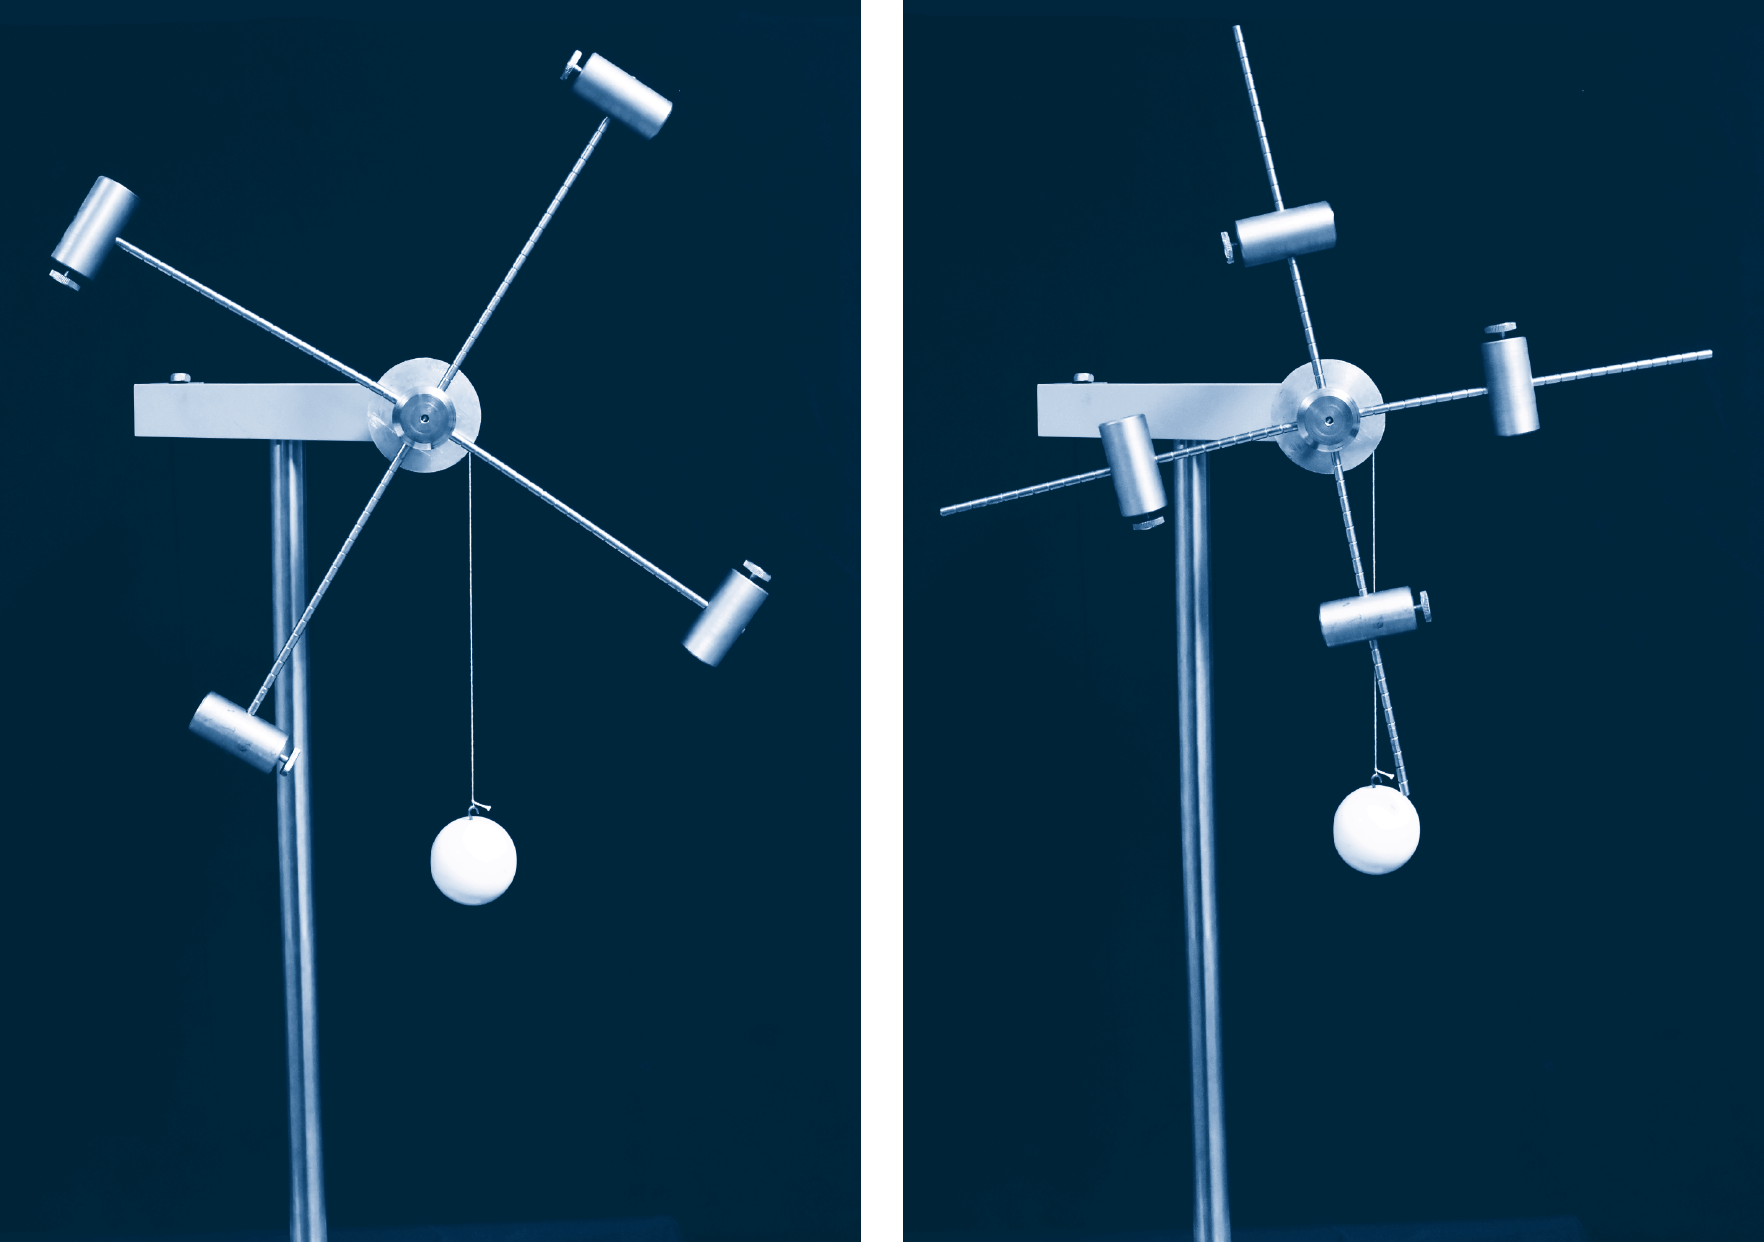
\includegraphics[width=0.9\linewidth]{oberbeck-1.png}
		\caption{Демонстрация инертных свойств тел при их вращении}
		\label{oberbeck-1}
	\end{figure}
	
	\subsection*{\underline{Оборудование:}}
	
	\begin{enumerate} 
		\item Крестообразный маятник с четырьмя грузами одинаковой массы, закрепленный на штативе.
		\item Шкив с перекинутой через него нитью.
		\item Тела различной массы, подвешенные на нити.
	\end{enumerate}

	\subsection*{\underline{Основные определения:}}
	
	Величина, которая одновременно учитывает влияние силы и ее 
	расположения относительно оси вращения на угловое ускорение 
	тела, называется моментом силы. 
	
	Расстояние \textit{r} от линии действия силы до оси вращения тела называют плечом силы. 
	
	Момент силы относительно оси считают равным произведению модуля силы на ее плечо: $$ M=Fr. $$
	
	Принято считать момент силы положительным, если он стремится вызывать вращение тела по часовой стрелке, и отрицательным — когда вызываемое им вращение имеет противоположное направление. 
	
	Согласно основному уравнению динамики вращательного движения угловое ускорение тела прямо пропорционально моменту действующих сил: $$ \varepsilon \sim M. $$
	Этот важный вывод подтверждается множеством опытов с вращением тел.
	
	Инертность тела по отношению к вращательному движению, ее влияние на угловое ускорение зависит не только от массы тела, но и от того, как она распределена относительно оси вращения. 
	Это означает, что на инертность во вращательном движении влияют форма и геометрические размеры тела, его расположение относительно оси вращения, в особенности распределение массы по объему тела. 
	
	Величина, которая определяет инертность тела по отношению к вращательному движению, называется моментом инерции тела.
	В механике различают осевые и центробежные моменты инерции. 
	
	Немецкий физик А. Обербек (1846-1900) известен как создатель механического устройства в виде крестовины с закрепленными на ее концах грузами, применяемого для изучения вращательного движения.

		\subsection*{\underline{Краткое описание:}}
		
	\textit{Опыт 1}. 
	Можно показать различный характер вращения тела с различными осевыми моментами инерции приводя во вращение в воздухе коробку или кусок пенопласта вокруг главных осей инерции.
	Для прямоугольного параллелепипеда главные оси инерции — это оси, проходящие через центры противоположных граней.
	Если подбросить кусок поролона, заставив его вращаться вокруг одной из осей инерции, то в отсутствие внешних сил можно заметить, что устойчиво вращение относительно главных осей, соответствующих наибольшему и наименьшему моментам инерции тела.
	Вращение вокруг главной оси, соответствующей среднему моменту инерции, будет неустойчиво.

	Вообще, практически оказывается, что вращение устойчиво вокруг оси с наибольшим моментом инерции.
	Это связано с влиянием внешних сил, в частности сил трения, которые создают момент относительно центра тяжести.
	Действие этого момента в случае вращения вокруг оси с наибольшим моментом инерции оказывается меньшим.
	
		\begin{figure}[H] 	
		\centering 	
		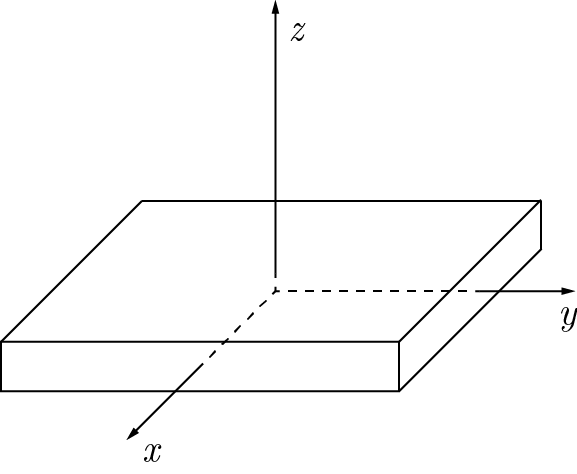
\includegraphics[width=0.45\linewidth]{oberbeck-2.png}
		\caption{Тело в форме прямоугольного параллелепипеда может обладать различными моментами инерции вокруг каждой из трех главных осей, характер вращения тела вокруг этих осей различается}
		\label{oberbeck-2}
	\end{figure}

	\textit{Опыт 2}. Маятник Обербека состоит из двух взаимно перпендикулярных стержней, вращающихся вокруг горизонтальной оси.
На стержни насажены четыре груза одинаковой массы, перемещение которых изменяет в довольно широких пределах момент инерции прибора. 
На оси прибора также находятся шкив, на который наматывается нить.
Подвесив к другому концу нити груз, можно создать вращающий момент и раскрутить маятник (рис.\ref{oberbeck-3}, \textit{а}).
И наоборот, вращая маятник с грузами можно, наматывая шнурок на шкив, поднимать груз.

Если грузы на стержнях маятника расположены близко к оси вращения, то момент инерции прибора невелик и скорость его вращения быстро достигает значительной величины (рис.\ref{oberbeck-3},\textit{б}).
Если же грузы сдвинуть к концам стержней, то момент инерции прибора возрастет; при этом он будет медленно набирать скорость и груз коснется пола спустя заметно большее время.

Опыт можно повторить, подвесив за нить груз большей массой.
Такой подход позволит изменить величину момента силы, действующей на маятник Обербека (положение грузов на спицах при этом менять не нужно), а, следовательно и характер вращения такого маятника.
	
	\begin{figure}[H] 	
		\centering 	
		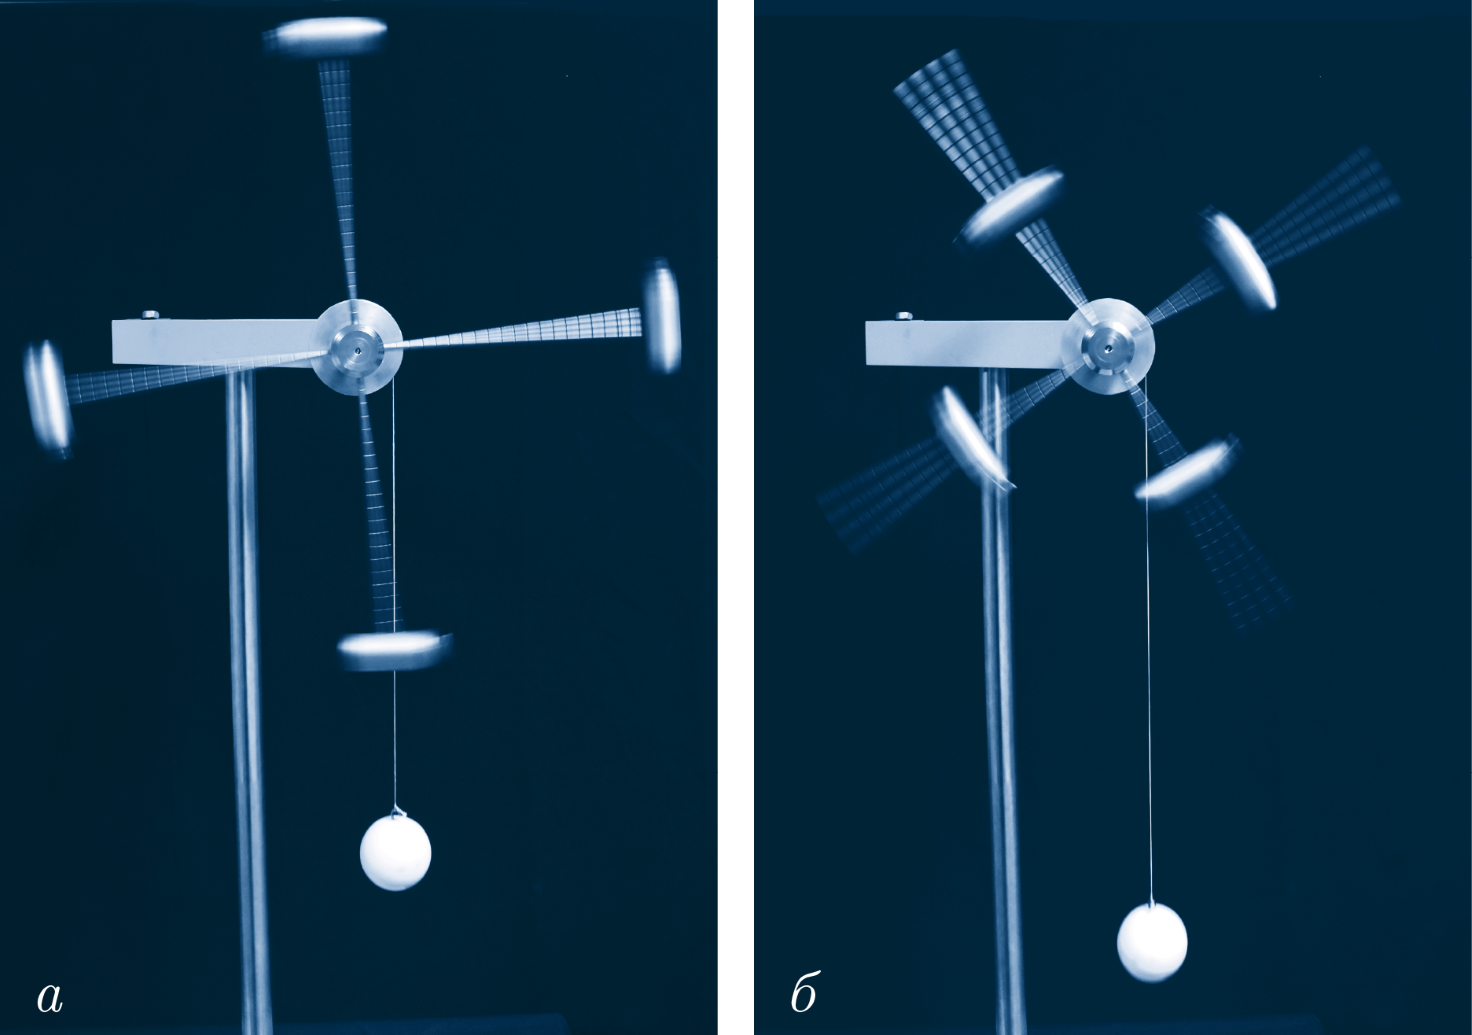
\includegraphics[width=0.8\linewidth]{oberbeck-3.png}
		\caption{Вращение крестообразного маятника Обербека при изменении момента инерции системы (\textit{а} и \textit{б})}
		\label{oberbeck-3}
	\end{figure}
	
	\subsection*{\underline{Теория:}}
	
Рассмотрим вращение крестообразного маятника Обербека при различном положении грузов \textit{m} относительно оси вращения (рис.\ref{oberbeck-4},\textit{а}), и с различной нагрузкой на шкив со стороны тела, подвешенного за нить (рис.\ref{oberbeck-4},\textit{б}). 
	
Запишем уравнение вращательного движения маятника вокруг неподвижной оси, считая, что нить невесома и нерастяжима, и пренебрегая силами трения:
\begin{equation}\label{oberbeck-eq1}
	I\varepsilon = M,
\end{equation}
где $ M=rT $ — момент внешних сил (в частности, силы натяжения нити \textit{T}), $ \varepsilon = \frac{\Delta\omega}{\Delta t} $ — угловое ускорение, $ \omega $ — угловая скорость, а $ I $ — момент инерции маятника Обербека.


	После подстановки момента силы натяжения нити уравнение вращательного движения маятника в проекции на ось \textit{z} можно записать как:
	\begin{equation}\label{oberbeck-eq2}
	I\varepsilon = rT. 
	\end{equation}

	\begin{figure}[H] 	
	\centering 	
	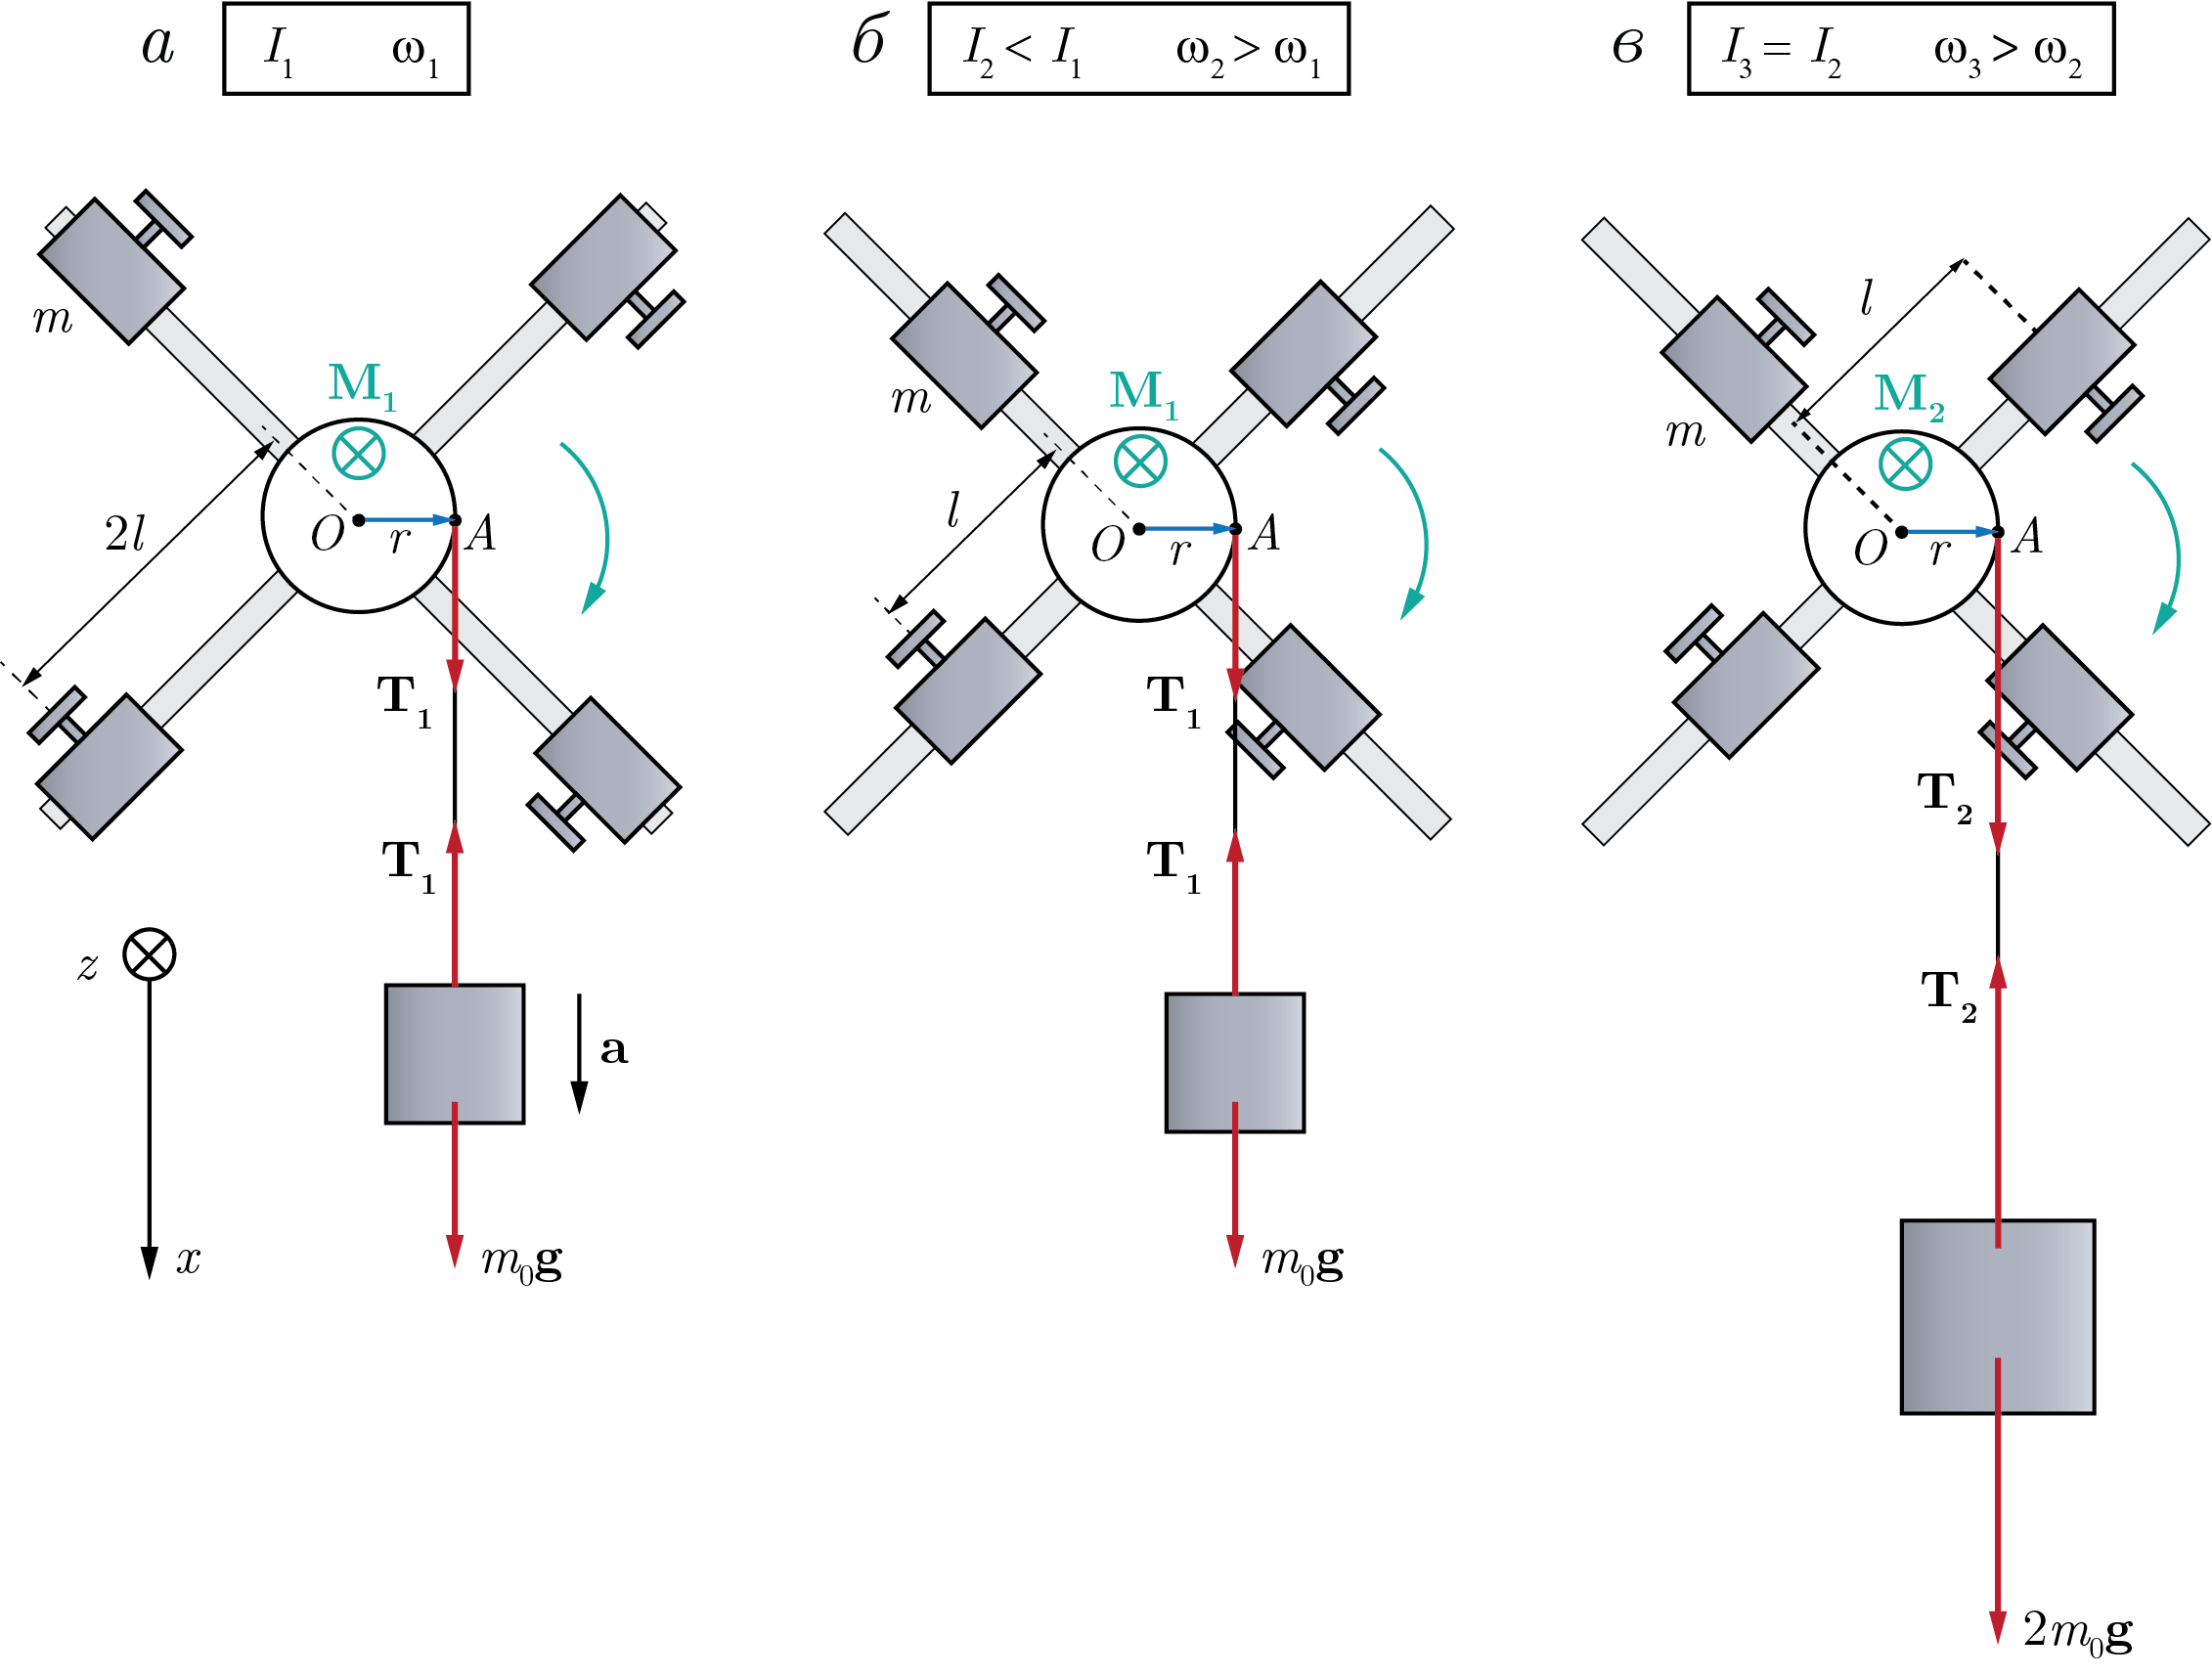
\includegraphics[width=0.9\linewidth]{oberbeck-4.png}
	\caption{Угловое ускорение креста Обербека зависит от расположения массы системы относительно оси вращения (\textit{а} и \textit{б}), а также от величины приложенной внешней силы (\textit{а} и \textit{в})}
	\label{oberbeck-4}
\end{figure}
	
	Второй закон Ньютона для поступательного движения большого груза в проекции на ось \textit{x} имеет следующий вид:
	\begin{equation}\label{oberbeck-eq3}
	m_0a = m_0g - T.
	\end{equation}
	Из связи линейного и углового ускорений точек вращающегося шкива имеем:
	\begin{equation}\label{oberbeck-eq4}
	a = r\varepsilon.
	\end{equation}
	Из уравнения (\ref{oberbeck-eq2}), выразим силу натяжения и воспользуемся соотношением (\ref{oberbeck-eq4}):
	\begin{equation}\label{oberbeck-eq5}
	T = \frac{I\varepsilon}{r} = \frac{Ia}{r^{2}}.
	\end{equation}
	Подставим полученное выражение в уравнение \ref{3}
	\begin{equation}\label{oberbeck-eq6}
	m_0a + \frac{Ia}{r^{2}} = m_0g.
	\end{equation}
	
	Домножая последнее выражение на $ r^{2} $
	\begin{equation}\label{oberbeck-eq7}
	a(m_0r^{2} + I) = m_0gr^{2}.
	\end{equation}
	можно получить соотношение для линейного ускорения $ a $:
		\begin{equation}\label{oberbeck-eq8}
	a = \frac{m_0gr^{2}}{m_0r^{2} + I},
	\end{equation}
	где $ I $ — момент инерции крестообразного маятника.
	
   Рассмотрим несколько конфигураций маятника Обербека.
            
  При неизменной массе грузов и радиуса шкива, будем менять расстояние между грузами массой $ m $ и осью вращения $ O $.
    Опыт показывает что, приближая грузы к оси вращения, при постоянном моменте внешней силы $ F_{\text{тяж}} $ маятник начинает раскручиваться с большим ускорением.
    Наблюдаемый эффект можно объяснить на основании теоремы Гюйгенса–Штейнера: 
    \begin{equation}\label{oberbeck-eq9}
    I = I_{0} + \sum_{i = 1}^{4}(I_{i}+m_{i}l_{i}^{2}),
    \end{equation}
    где $ I_{0} $ — момент крестообразного маятника без грузов на стрежнях.
    
    Из полученного соотношения видно, что при приближении грузов к оси вращения, момент инерции маятника уменьшается, то есть $ I_2<I_1 $.
    И наоборот, с ростом $ l $ момент инерции увеличивается.
    Таким образом, на рис.\ref{oberbeck-4},\textit{а} момент инерции больше, чем во втором случае (рис.\ref{oberbeck-4},\textit{б}).
    
    Отсюда следует, что при постоянном значении момента внешней силы вращающиеся тела тем быстрее изменяют свою угловую скорость, чем меньше их момент инерции.
		
 При неизменном положении $ l $ грузов на крестовине, можно увеличить внешнюю силу, и, соответственно, создать больший момент силы (рис.\ref{oberbeck-4},\textit{в}). 
	Угловое ускорение маятника в этом случае также окажется больше, чем в случае на рис.\ref{oberbeck-4},\textit{б}.
	Возрастет кроме этого и линейное ускорение массивного тела, создающего этот самый момент силы.
	Такая зависимость углового ускорения маятника от прикладываемого внешнего момента силы выражается соотношением (\ref{oberbeck-eq8}).  

\end{document}
